\documentclass[12pt]{article}
\usepackage{mathematics}

\begin{document}

\begin{mdframed}
  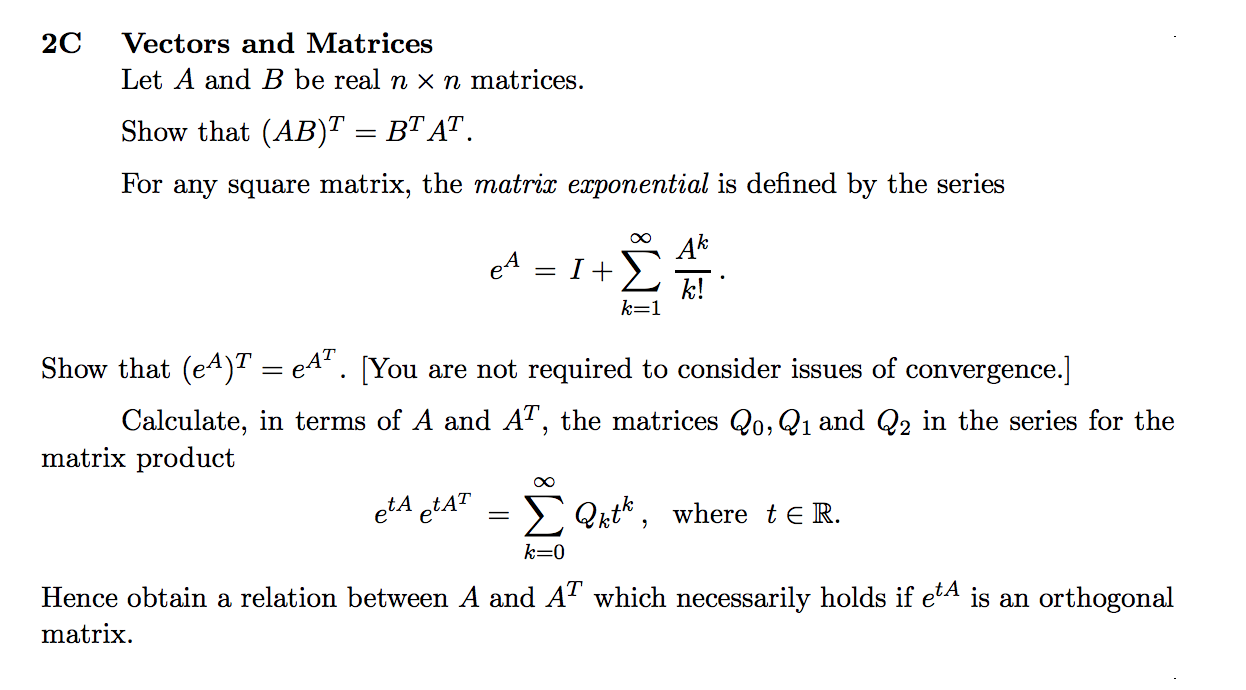
\includegraphics[width=400pt]{img/misc--cambridge-1a-2017-1-2c.png}
\end{mdframed}

\begin{claim*}
  $(AB)^T = B^TA^T$
\end{claim*}

\begin{proof}
  Let $i, j \in \{1, \ldots, n\}$. Then
  \begin{align*}
    \((AB)^T\)_{ij} &= (AB)_{ji}\\
                    &= \sum_{l=1}^n A_{jl}B_{li}\\
                    &= \sum_{l=1}^n (A^T)_{lj}(B^T)_{il}\\
                    &= (B^TA^T)_{ij}
  \end{align*}
\end{proof}

\begin{lemma*}
  $(A^k)^T = (A^T)^k$.
\end{lemma*}

\begin{proof}
  Note that $(A^k)^T = (AA^{k-1})^T = (A^{k-1})^TA^T$. Repeating this procedure proves the lemma.
\end{proof}

\newpage
\begin{claim*}
  $(e^A)^T = e^{(A^T)}$
\end{claim*}

\begin{proof}
  Note that $(e^A)_{ij} = \sum_{k=0}^\infty \frac{(A^k)_{ij}}{k!}$, where $A^0 := I$ and $0! := 1$.
  Therefore
  \begin{align*}
    \((e^A)^T\)_{ij} &= \sum_{k=0}^\infty \frac{((A^k)^T)_{ij}}{k!} ~~~~~~\text{and}\\
    (e^{(A^T)})_{ij} &= \sum_{k=0}^\infty \frac{((A^T)^k)_{ij}}{k!},
  \end{align*}
  and it will suffice to show that these are equal.

  For example, let $A = \matMMxNN{a}{b}{c}{d}$. Then
  \begin{align*}
    A^T        &= \matMMxNN{a}{c}
                           {b}{d}\\
    A^2        &= \matMMxNN{a^2 + bc}{ab + bd}
                           {ac + cd}{bc + d^2}\\
    (A^2)^T    &= (A^T)^2 = \matMMxNN{a^2 + bc}{ac + cd}
                                     {ab + bd}{bc + d^2}.
  \end{align*}
\end{proof}

\begin{claim*}
  $$
\end{claim*}

\begin{proof}
  \begin{align*}
    (A^k)^T &= (AA^{k-1})^T\\
            &= (A^{k-1})^TA^T
  \end{align*}
\end{proof}

\end{document}
